\documentclass[aps,prb,twocolumn,groupedaddress,notitlepage,showpacs,floatfix,superscriptaddress]{revtex4-1}
\usepackage{times,amsmath,amsfonts,amssymb,mathrsfs,graphics,graphicx,color,comment,bm}
\usepackage[dvips]{epsfig}
\usepackage[pdfstartview=FitH]{hyperref}
\usepackage{natbib}
\usepackage{appendix}
\usepackage{epstopdf}
\usepackage[export]{adjustbox}
\hypersetup{
colorlinks=true,       	
linkcolor=blue,          	
citecolor=blue,        
filecolor=blue,      	
urlcolor=blue,           	
runcolor=blue
}
\newcommand{\ignore}[1]{}
%%%%%%%%%%%%%%%%%%%%%%%%%%%%%%%%%%%%%%%%%%%%%%%%%%%%%%%%%%%%%%%%
\let\oldsqrt\sqrt
\def\sqrt{\mathpalette\DHLhksqrt}
\def\DHLhksqrt#1#2{%
\setbox0=\hbox{$#1\oldsqrt{#2\,}$}\dimen0=\ht0
\advance\dimen0-0.2\ht0
\setbox2=\hbox{\vrule height\ht0 depth -\dimen0}%
{\box0\lower0.4pt\box2}}

%%%%%%%%%%%%%%%%%%%%%%%%%%%%%%%%%%%%%%%%%%%%%%%%%%%%%%%%%%%%%%%%
% in: s * [x], "x" is the magnification factor
\DeclareFontFamily{OT1}{pzc}{}
\DeclareFontShape{OT1}{pzc}{m}{it}%
              {<-> s * [1.25] pzcmi7t}{}
\DeclareMathAlphabet{\mathpzc}{OT1}{pzc}%
                                 {m}{it}
%%%%%%%%%%%%%%%%%%%%%%%%%%%%%%%%%%%%%%%%%%%%%%%%%%%%%%%%%%%%%%%%
%%%%%%%%%%%%%%%%%%%%%%%%%%%%%%%%%%%%%%%%%%%%%%%%%%%%%%%%%%%%%%%%

\begin{document}
\title{Unitary Tensor Network Ansatz for May-body localized Hamiltonians}
\author{R. Haghshenas}
%\affiliation{Department of Physics, Sharif University of Technology, P. O. Box
%11155-9161, Tehran, Iran}
%\email{haghshenas@physics.sharif.edu}
%\date{\today}
%\begin{abstract}
%\end{abstract}
\maketitle

%%%%%%%%%%%%%%%%%%%%%%%%%%%%%%%%%%Fig. 2%%%%%%%%%%%%%%%%%%%%%%%%%%%%%%%%%%%%%%%%%%
\begin{figure}
  \begin{centering}
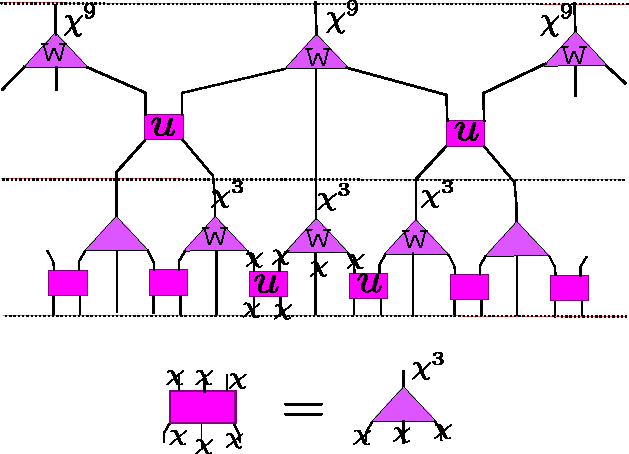
\includegraphics[width=1.0 \linewidth]{MERA-MBL}  \end{centering}
  \caption{(Color online) Tensor Network representation of $MUTNA$ in terms of local tensors $\{u, w\}$. all tensors are constrained to be unitary.}
  \label{fig:MERA}
\end{figure}
 %%%%%%%%%%%%%%%%%%%%%%%%%%%%%%%%%%%%%%%%%%%%%%%%%%%%%%%%%%%%%%%%%%%%%%%%5

We introduce a MERA-like Unitary Tensor Network Ansatz ($MUTNA$) to obtain full spectrum of many-body localized Hamiltonians. The goal here is to represent the unitary $U$, which diagonalizes many-body localized Hamiltonian, in terms of local tensors, i.e. $\{u, w\}$. As depicted in Fig.~\ref{fig:MERA}, e.g., a two-layer Ternary $MUTNA$ is consist of tensors $u$ and $w$, where each tensor is constrained to be Unitary that guarantees the Ternary $MUTNA$ also to be itself unitary. Note that here, in contrast to MERA for ground-state optimization, there is no truncation at all.      

The local tensors $\{u, w\}$ is obtained by minimizing the cost function $\sigma^{2}$, i.e.,
\begin{equation*}
\sigma^{2}(\{u, w\})=\mathrm{Tr}(H^{2})-\sum_{i=1}^{2^{N}} (U^{\dagger}(u, w)HU(u, w))^{2}_{(i,i)}
\end{equation*}
where $H$, $U(u,w)$ and $N$ respectively stand for many-body localized Hamiltonian, $MUTNA$ and number of particles. The method/algorithm for minimizing/maximizing the cost function $\sigma^{2}(\{u, w\})$ has been before described in details in our previous communications. Optimization scheme  centres on two methods, (1) linearizing cost function in terms of tensors and then updating them (similar to that of MERA optimization), however this methods does not always guarantee to converge to true minimum/maximum value and (2) Using steepest descent method which always find `local' minimum or maximum of cost function. In our simulation, we use both of them to make sure optimization result in true minimum/maximum, but note that optimization based on linearizing is much more quicker. We point out the novel futures of $MUTNA$.
%%%%%%%%%%%%%%%%%%%%%%%%%%%%%%%%%%%%%%%%%%%%%%%%%%%%
\begin{table}[tp]
\caption{
 Accuracy of $MUTNA$ for Heisenberg Model (averaged over a number of realization to obtain converged value).
}
\begin{ruledtabular}
\begin{tabular}{lrrrr}
$W$&$N$& $\overline{\sigma^{2}}/2^{N}$ &
Complexity\\
\colrule
$8$ & $10$ & $1.4\times10^{-3}$ & $\mathcal{O}(2^{18})$   \\
$6$ & $10$ & $2.5\times10^{-3}$ & $\mathcal{O}(2^{18})$  \\
$8$ & $18$ & $9\times10^{-4}$ & $\mathcal{O}(2^{27})$ \\
$6$ & $18$ & $2.7\times10^{-3}$ & $\mathcal{O}(2^{22})$ \\
\end{tabular}
\end{ruledtabular}
\label{table-1}
\end{table}
%%%%%%%%%%%%%%%%%%%%%%%%%%%%%%%%%%%%%%%%%%%%%%%%%%%%

%%%%%%%%%%%%%%%%%%%%%%%%%%%%%%%%%%Fig. 2%%%%%%%%%%%%%%%%%%%%%%%%%%%%%%%%%%%%%%%%%%
\begin{figure}
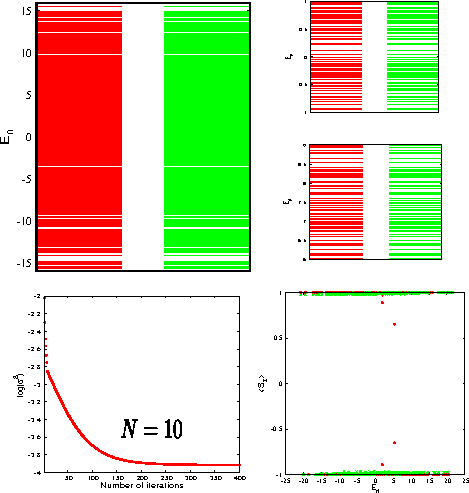
\includegraphics[width=1.0 \linewidth]{Data}  
  \caption{(Color online) red and green colors respectively stand for exact diagonaliztion and $MUTNA$. The energy spectrum $E_{n}$, magnetic order $S_{z}$ and energy accuracy $\log_{10}(\sigma^{2})/2^{N}$ has been calculated for $N=10$.     }
  \label{fig:Data}
\end{figure}
 %%%%%%%%%%%%%%%%%%%%%%%%%%%%%%%%%%%%%%%%%%%%%%%%%%%%%%%%%%%%%%%%%%%%%%%%5


\begin{itemize}
\item Since the method/algorithm does not require matrix product operator representation for Hamiltonian, it could be applied to one- and two-dimensional local Hamiltonians. Actually, it only exploits locality of Hamiltonians, and therefore any MERA scheme for obtaining ground state---such as binary/Ternary/Modified binary and also two-dimensional versions---could be used to obtain full spectrum.    

\item Similar to that of scale invariant MERA, which address the models in thermodynamics limit, one could construct similar scheme to study many-body localization for $N\rightarrow \infty$. Especially, in case of translational invariant models showing many-body localization, the scale invariant $MUTNA$ could be helpful.

\item Time complexity of algorithm scales like $\mathcal{O}(\chi^{9})$ for `Ternary $MUTNA$', where $\chi$ is bond dimension of tensors at the last layer. Bond dimension $\chi$ actually increase as $2^{i}$, where $ i \in ( 1,2,\cdots )$. For Binary and Modified Binary $MUTNA$, time complexity scales like respectively $\mathcal{O}(\chi^{10})$ and $\mathcal{O}(\chi^{8})$, but however, Binary $MUTNA$ produces much more entanglement which might be more accurate. A combination of all schemes is also possible.       
\end{itemize} 

We report some of our results for the the Heisenberg model with random fields in one dimension,
\begin{equation*}
H= \sum_{i}\overrightarrow{S}_{i}\cdot\overrightarrow{S}_{i+1}-h_{i}S^{z}_{i}
\end{equation*}
where $\overrightarrow{S}$ are spin-$1/2$ operators and random fields $h_{i}$ are determined from interval $[-W,W]$. Fig.~\ref{fig:Data} compares the results of exact diagonalization (red color) versus $MUTNA$ (green color) and also speed of energy convergence for the following realization,
\begin{align*}
h=(0.82,-7.3,-4.9,7.1,-0.32,-6.1,-7.1,3.5,-3.4,-0.70),
\end{align*}
where number of spins $N=10$ and $\sigma^{2}/2^{N}=62.9865-62.9864=1.3\times10^{-4}$. Another case study for $N=18$ spins is 
\begin{align*}
h=&(-2.14,4.82,1.85,1.62,-5.79,4.12,-0.72,-0.90,2.27,-2.73, \\
&-4.55,1.03,-4.48,5.58,3.63,-1.31,1.17,-3.33),
\end{align*}
where in this case $\sigma^{2}/2^{N}=52.97508-52.97484=2.40\times10^{-4}$. Table.~\ref{table-1} reports accuracy of $MUTNA$ ($\overline{\sigma^{2}}/2^{N}$ is averaged over a number of realizations to converge to a specific vale) for different disorder and number of spins.


%%%%%%%%%%%%%%%%%%%%%%%%%%%%%%%%%%Fig. 2%%%%%%%%%%%%%%%%%%%%%%%%%%%%%%%%%%%%%%%%%%
\begin{figure}[t]
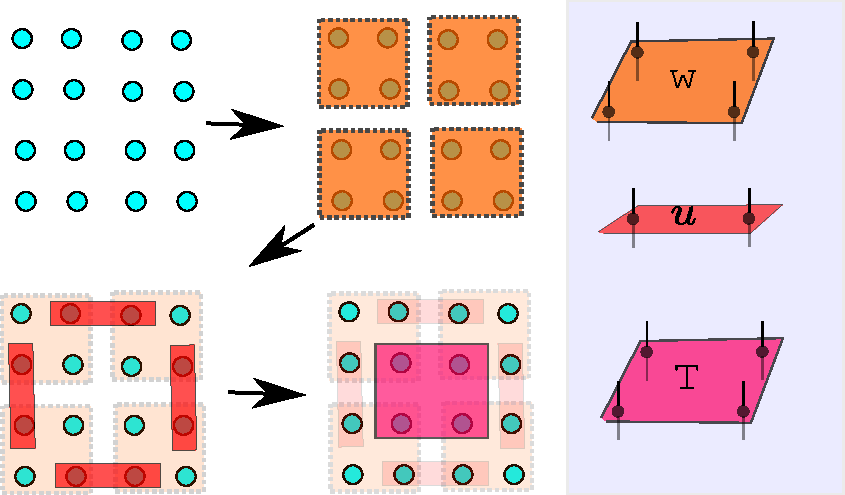
\includegraphics[width=1.0 \linewidth, left]{MERA2D} 
  \caption{(Color online) $MUTNA$ scheme for a square lattice. We apply unitary $\{u, w, T\}$ accordingly to remove all short-range entanglement between spins. Actually, with this scheme, we guarantee that each state of model respects the area law.}
  \label{fig:MERA2D}
\end{figure}
 %%%%%%%%%%%%%%%%%%%%%%%%%%%%%%%%%%%%%%%%%%%%%%%%%%%%%%%%%%%%%%%%%%%%%%%%5
 

We propose a two-dimensional $MUTNA$, as depicted in Fig.~\ref{fig:MERA2D}, to address two-dimensional many-body localized Hamiltonian. The $MUTNA$ is consisted of three unitary tensors $\{u, w, T\}$ applied consequently according to Fig.~\ref{fig:MERA2D}. Each one has been designed to removes short-range entanglements between the sites (please note how much the tensor network structure is similar to that of MERA for 2-dimensional cases). We could apply $MUTNA$ for the square lattice of size $\{4\times4,5\times5,6\times6\}$---Simulation of such sizes with today's computers (a desktop computer) could be done in a reasonable time. For these cases, the complexity is of order $\mathcal{O}(\chi^{12})$. We have developed our code and tested the algorithms and obtained some preliminary results, but the work is in progress and needs much more discussion (about the physics of such systems) and also computational techniques.

        
\bibliography{references} 
 
\end{document}

